%% ------------------------------------------------------------------------- %%
\chapter{Planejamento do Experimento}
\label{cap:planejamento}

Conforme discutido no Capítulo \ref{cap:trabalhos-relacionados}, muitos 
trabalhos avaliaram TDD, e alguns deles relatam uma melhora
no design de classes, como um menor acoplamento, uma maior coesão, e até mesmo
mais simplicidade nas classes quando desenvolvidas utilizando-se a prática. 
Grande parte deles estão interessados em avaliar quais os efeitos da prática
no código final produzido, mas poucos estudos tentam entender como TDD e a
prática de escrever o teste antes do código real realmente guiam o programador 
em direção à essas melhorias.

Para entender como TDD influencia as decisões do desenvolvedor durante o desenvolvimento,
este trabalho propõe estudos de caso em empresas de desenvolvimento de
software brasileiras, utilizando métodos qualitativos de pesquisa.
Este capítulo detalha o planejamento do experimento, bem como o processo de
análise dos dados colhidos.

%% ------------------------------------------------------------------------- %%
\section{Design da pesquisa}

Baseando-se no fato de que o processo de desenvolvimento de software envolve 
diversos fatores humanos e é totalmente sensível ao contexto em que ele está 
inserido, este trabalho é composto por um \textbf{conjunto de estudos de caso},
onde são utilizados métodos qualitativos de pesquisa para o processo de colheta e 
análise dos dados.

Segundo a definição de Robson \cite{robson}, Yin \cite{yin} e Benbasat et
al. \cite{benbasat}, Runeson e Host mostram que todas as definições concordam
que um estudo de caso investiga um fenômeno contemporâneo no seu contexto. 
Robson afirma que um estudo de caso estressa o uso de múltiplas fontes de
evidência, Yin denomina estudo de caso um "inquérito" e destaca que os limites 
entre o fenômeno e seu contexto podem não ser claros, enquanto que Benbasat et
al. menciona que um estudo de caso recolhe informações de poucas entidades 
(como pessoas, grupos ou organizações) e que também é caracterizado pela falta
de controle experimental \cite{guidelines-case-study}.

A intenção dos estudos de caso é obter informações relevantes sobre como os
praticantes de TDD utilizam a prática para influenciar o design de suas
classes. Na tentativa de capturar o máximo de informações possíveis, esse estudo
inclui uma análise profunda através de entrevistas, observações no mundo real e 
avaliação de métricas de código.

%% ------------------------------------------------------------------------- %%
\section{Participantes da pesquisa}
\label{sec:planejamento-participantes}

Para a condução do estudo de caso, algumas empresas do mercado de software
brasileiro foram selecionadas de acordo com alguns critérios.
Os critérios que foram levados em consideração no momento de convidar empresas a
participarem da pesquisa foram:

\begin{itemize}
	\item Programadores que utilizem de TDD há mais de 1 ano;
	
	\item Programadores que desenvolvam software há mais de 3 anos;

	\item Localizadas em São Paulo (SP), para facilitar o processo de
	entrevista e observação do ambiente;

	\item Desenvolvedores com diferentes níveis de experiência em TDD e em 
	Orientação a Objetos, desde iniciantes até experientes;

	\item Projetos que utilizem a tecnologia Java e sejam baseados na web;

	\item Metodologias ágeis como processo de desenvolvimento de
	software;
\end{itemize}

Ao final, três empresas foram selecionadas. Todas elas desenvolvem softwares de
pequeno e médio porte (e por isso entenda-se software entre 100 a 500 mil linhas
de código), utilizando a plataforma Java para desenvolvimento. Elas também 
possuem profissionais com os mais variados níveis de experiência na área 
trabalhando juntos no mesmo time.

A repetição do experimento em diferentes empresas com diferentes projetos,
equipes e contextos serve como estratégia de validação dos resultados
encontrados.

%% ------------------------------------------------------------------------- %%
\section{Estratégia de pesquisa} 
\label{sec:planejamento-estrategia}


Os dados serão coletados principalmente através de entrevistas com
desenvolvedores que praticam TDD no dia-a-dia de trabalho e que podem avaliar
com propriedade o efeito da prática sobre o design orientado a objetos dos seus 
projetos, durante os meses de Junho e Agosto de 2011. 
Além disso, o ambiente será observado pelo pesquisador afim de capturar
informações do cotidiano relevantes para a pesquisa.

As sub-seções abaixo detalham como os dados serão colhidos em cada etapa da pesquisa.

%% ------------------------------------------------------------------------- %%
\subsection{Entrevistas}
\label{sec:planejamento-estrategia-entrevistas}

O primeiro passo da pesquisa é uma série de entrevistas com os desenvolvedores 
das empresas participantes, que serão realizadas entre os meses de Junho e
Julho de 2011. As entrevistas serão semi-estruturadas, dando liberdade ao
pesquisador para mudar o rumo das perguntas, caso se faça necessário.

Além disso, todas as perguntas serão abertas, permitindo que o desenvolvedor dê
uma resposta ampla sobre o assunto. A tabela \ref{tab:questoes} mostra a
relação entre os objetivos da entrevista e as perguntas formuladas no roteiro de
entrevista, encontrado no apêndice \ref{ape:entrevista} deste trabalho.

\begin{table}[h!]
	\begin{tabular}{ | p{6cm} | p{7cm} | p{2cm} | }
		\hline
		\textbf{Caracterizar a experiência do programador com desenvolvimento de
		software, boas práticas de desenvolvimento e TDD} 
		&
		Vital para caracterizar o público-alvo da pesquisa.
		&
		Seções \ref{entrevista:dados-basicos}, \ref{entrevista:caracterizacao}
		\\

		\hline
		\textbf{A relação entre a experiência do programador e os efeitos de TDD
		na qualidade do design} 
		&
		Por ser um outro possível fator de influência, o pesquisador colherá
		informações sobre a experiência do programador com desenvolvimento de softwares, 
		conceitos de orientação a objetos e TDD.
		&
		Seções \ref{entrevista:experiencia}
		\\

		\hline
		\textbf{Como o desenvolvedor vê a influência que a utilização de TDD
	junto com outras práticas ágeis, como programação pareada, tem sobre o design} 
		&
		Por ser um possível fator de influência, o pesquisador colherá informações
		para diferenciar efeitos da programação pareada dos efeitos de TDD.
		&
		Seções \ref{entrevista:tdd-e-praticas-ageis}
		\\

		\hline
		\textbf{A visão do desenvolvedor sobre a influência de TDD no design} 
		&
		O pesquisador alinhará as definições da prática com todos os participantes da
		pesquisa.
		&
		Seções \ref{entrevista:pratica}
		\\

		\hline
		\textbf{Os efeitos de TDD sobre o acoplamento e a coesão geral das classes do
		sistema} 
		&
		Entender a opinião do participante sobre os efeitos de TDD
		nesses dois pontos importantes em sistemas orientados a objetos.
		&
		Seções \ref{entrevista:acoplamento}, \ref{entrevista:coesao}
		\\

		\hline
		\textbf{Os efeitos de TDD sobre a gerenciamento de dependências em
		sistemas orientados a objetos} 
		&
		Em um nível maior, entender qual a possível influência da prática no
		gerenciamento de dependências. 
		&
		Seções \ref{entrevista:dependencias}
		\\

		\hline
		\textbf{Como o desenvolvedor utiliza o feedback dos testes para guiar o
		design} 
		&
		Entender como o desenvolvedor utiliza os testes para melhorar o design
		e, para isso o pesquisador perguntará desde questões conceituais até questões
		bem práticas com discussões de trechos de código.
		&
		Seções \ref{entrevista:tdd-guiar-design}
		\\

		\hline
		\textbf{A relação entre TDD e boas práticas de orientação a objetos} 
		&
		O pesquisador colherá informações sobre a relação entre a prática e
		bons princípios de orientação a objetos, como SOLID \cite{bob-martin}.
		&
		Seções \ref{entrevista:tdd-guiar-design}
		\\

		\hline
		\textbf{A visão do programador sobre a simplicidade que TDD agrega ao
		processo} 
		&
		Entender como TDD leva o programador à criação de códigos mais simples.
		&
		Seções \ref{entrevista:simplicidade}
		\\
		
		\hline												
	\end{tabular}
	\caption{Relação entre os objetivos e as perguntas da entrevista.}
	\label{tab:questoes}
\end{table}

O processo de entrevista será composto por uma breve introdução da pesquisa, de
modo a não enviesar o participante, seguida de algumas perguntas que visam
caracterizar o perfil do participante; perguntas como qual a experiência do
desenvolvedor em desenvolvimento de software e TDD são necessárias para ajudar o
pesquisador no entendimento das respostas dadas. Além disso, perguntas sobre
referencias, livros e outros pontos de informação nas quais o participante lê a
respeito da prática servem para que o programador entenda o embasamento teórico
do praticante sobre TDD.

Em seguida, o pesquisador perguntará os pontos discutidos na listagem anterior.
Para isso, o pesquisador fará uso não só de perguntas abertas, mas também
solicitará exemplos de código, para que as respostas se tornem técnicas e
específicas. O pesquisador solicitará ao participante que rascunhe pequenos
trechos de código durante a discussão, e essas anotações serão anexadas junto ao
conjunto de dados colhetados da pesquisa.
Por fim, o pesquisador pedirá referências ao pesquisador sobre
possíveis próximos entrevistados, afim de descobrir os programadores referencias 
na prática para aquele determinado participante.

Todas as entrevistas serão gravadas, para que o pesquisador possa fazer a
transcrição e rever os dados a qualquer momento durante o processo. Além disso,
o pesquisador também tomará notas, capturando informações como reações dos 
participantes a determinadas perguntas, ou qualquer outra informação relevante. 

As entrevistas serão feitas em dias diferentes para que, ao final
de cada dia, o pesquisador possa discutir sobre os pontos levantados no dia
corrente e sugerir melhorias no instrumento de pesquisa. 
O processo de codificação será feito por dois
pesquisados separadamente, e só então ambos juntarão seus resultados, após uma 
série de comparações e discussões sobre as diferenças encontradas.

%% ------------------------------------------------------------------------- %%
\subsection{Observação do ambiente real}
\label{sec:planejamento-observacao}

O pesquisador observará os participantes durante suas atividades diárias. As
visitas serão pré-agendadas com os líderes técnicos de cada equipe, de modo a
otimizar o tempo, e evitar a presença do pesquisador durante atividades
não que não fazem uso da prática, como reuniões de trabalho.

O período mínimo de observação será de 2 horas. Após esse período, o observador
decidirá se o tempo de observação deverá ser prolongado. O número mínimo de
observações será de 10 por equipe, garantindo que cada equipe será observada por
no mínimo 20 horas de trabalho. Durante as observações, o pesquisador focará na
questão de pesquisa relacionada à \textit{como o teste guia o desenvolvedor
durante a atividade de design?}. Discussões sobre qualquer um dos pontos abaixo, 
mas não limitados a eles, serão capturadas pelo pesquisador:

\begin{itemize}
  
  \item A influência do teste ser o primeiro cliente da classe;

  \item A explícitação das dependências necessárias para a escrita do teste de
  unidade;

  \item Testes que mostram a falta de coesão de uma classe;

  \item A não criação de classes altamente acopladas;

  \item Criação de classes com menor tamanho;

  \item A utilização da técnica de composição de classes;
  
  \item A relação entre a dificuldade da escrita do teste e designs mais
  flexíveis;

\end{itemize}

Para auxiliar o processo de observação, o pesquisador tomará notas durante o
processo, e fará as perguntas que achar necessário para os participantes. Além
disso, o pesquisador observará também o código final produzido pelas equipes,
possibilitando assim o relacionamento entre a prática e a qualidade do design
final produzido.

%% ------------------------------------------------------------------------- %%
\subsection{Métricas de código}
\label{sec:planejamento-metricas}

Após o processo de entrevistas e observação, o pesquisador fará uso de métricas
de código para validar algumas das informações obtidas através das entrevistas e
observações. O objetivo nesse ponto é triangular com as informações obtidas
de maneira qualitativa. 

Para facilitar o entendimento e a interpretação, as métricas
serão calculadas em diferentes pontos do código-fonte dentro do controlador de versão,
possibilitando ao pesquisador uma análise sobre os efeitos de TDD no design ao
longo do tempo. Além disso, as métricas não serão avaliadas sozinhas, mas sim
através de uma soma de fatores. 
A Tabela \ref{tab:metricas} abaixo relaciona as métricas de código sugeridas com
as questões de pesquisa, bem como a maneira na qual serão avaliadas.

\begin{table}[h!]
	\begin{tabular}{ | p{5cm} | p{5cm} | p{5cm} | }
		\hline
		Questão de Pesquisa & Métrica & Avaliação \\
		
		\hline
		
		\multirow{4}{5cm}{Como a prática de TDD afeta o acoplamento das classes criadas?} 
		& Acoplamento Aferente & \multirow{4}{5cm}{O acoplamento não será avaliado
		apenas numericamente; classes serão declaradas como altamente acopladas ao
		não fazerem uso de princípios como DIP, OCP e LSP \cite{bob-martin}, que
		permitem com que classes sejam evoluídas de forma mais natural.} \\ & Acoplamento Eferente
		& \\ & Indícios de presença de DIP & \\ & Indícios de presença de OCP & \\
		& Indícios de presença de LSP & \\
		& & \\ & & \\ & & \\ & & \\
		\hline
		
		\multirow{3}{5cm}{Como a prática de TDD afeta o gerenciamento de dependências em sistemas
		orientados a objetos?} 
		& Instabilidade & 
		\multirow{3}{5cm}{Seguindo o princípio de estabilidade \cite{bob-martin},
		acoplamentos também serão consideradas maléficos se forem feitos com classes menos abstratas 
		do que a classe em observação} \\ 
		& Abstração & \\ 
		& Distância da Linha Principal & \\
		& & \\ & & \\ & & \\ & & \\

		\hline
		
		\multirow{3}{5cm}{Como a prática de TDD afeta a coesão das classes criadas?} 
		& LCOM* & 
		\multirow{3}{5cm}{Classes serão consideradas não coesas caso a métrica de
		coesão seja maior do que 10 ou tiverem mais de 25 métodos
		públicos em sua interface} \\ 
		& Indícios de presença de SRP & \\ 
		& Indícios de presença de ISP & \\
		& Número de métodos na classe & \\
		& & \\ & & \\ & & \\
		\hline
		
		\multirow{2}{5cm}{Como TDD afeta a simplicidade das classes criadas?}
		& Número de linhas por método & 
		\multirow{4}{5cm}{Classes serão consideradas simples se a complexidade
		ciclomática por linha de código for menor do que 0.20 } \\
		& Complexidade ciclomática & \\
		& & \\ & & \\
		
		\hline
	\end{tabular}
	\caption{Métricas de código avaliadas na pesquisa}
	\label{tab:metricas}
\end{table}

Os valores para as métricas de coesão e quantidade de métodos públicos foram
derivadas do trabalho de Kecia et al \cite{kecia}, e os valores acima são médias
dos intervalos de valores considerados como ``regular''. Já os valores de
complexidade ciclomáticas foram baseados no valor considerado como ``médio'' no
trabalho de Lanza et al \cite{lanza}.

%% ------------------------------------------------------------------------- %%
\section{Análise dos dados}
\label{sec:planejamento-analise}

O processo de análise, baseado em \cite{creswell}, que está representado na
Figura \ref{fig:analise-dados}, ilustra o processo de análise que será utilizado
nessa pesquisa. Apesar de parecer uma abordagem em cascata, ele é na prática 
interativo, já que os passos são interconectados. 

A princípio, os dados serão preparados, através das transcrição das
entrevistas e das notas geradas durante as observações, além das
visualizações das métricas de código colhidas. A seguir, a leitura completa dos
dados colhidos para que o pesquisador possa buscar por erros no processo de
transcrição e para que reflita também sobre os principais pontos e opiniões em
todas as fontes de dados.

O processo de codificação e o agrupamento
por temas será então realizado, que por fim aparecerão como maiores
contribuições da pesquisa qualitativa, durante o processo de interpretação dos
dados pelo pesquisador. O software utilizado para o processo de codificação será
o \textit{Atlas.ti} \footnote{\url{http://www.atlasti.com/}. Último acesso em 3
de maio de 2011.}, produzido na Alemanha, que permite ao pesquisador organizar textos,
gráficos, aúdios, e arquivos visuais, e juntá-los com códigos e anotações. 

Durante todo o processo, o pesquisador constantemente validará toda e qualquer
informação colhida e, caso seja necessário, a colheta de qualquer entrevista,
observação ou métrica poderá ser refeita. Os participantes das entrevistas
são comunicados de que o pesquisador poderá entrar em contato
novamente para alguma eventual dúvida.

\begin{figure}
  \centering
  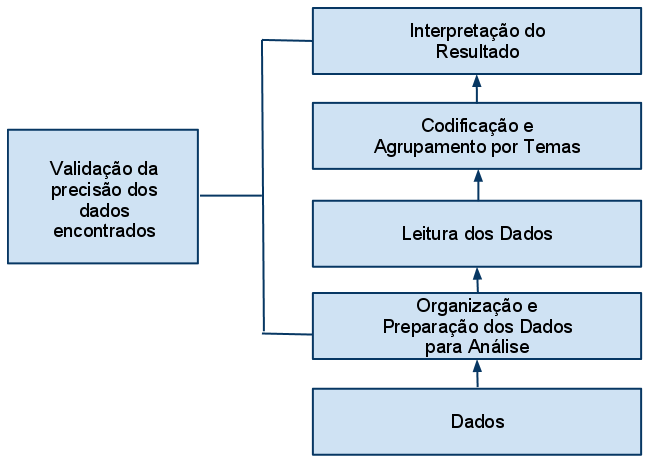
\includegraphics[scale=0.5]{analisedados}
  \caption{Processo de análise dos dados}
  \label{fig:analise-dados}
\end{figure}

 %% ------------------------------------------------------------------------- %%
\section{Validade e Confiabilidade do Estudo}
\label{sec:planejamento-validacao}

Para garantir a confiabilidade deste estudo, o pesquisador realizará os
seguintes procedimentos:

\begin{itemize}
	\item \textbf{Checar as transcrições}. O objetivo é garantir que nenhum erro
	óbvio foi cometido;

	\item \textbf{Verificação de pesquisador auxiliar}. Um pesquisador auxiliar
	checará se há algum desvio na definição dos códigos ou no significado dos códigos 
	durante o processo de codificação;
	
	\item \textbf{Rastreabilidade dos dados}. Todos os dados colhidos serão
	preservados em forma eletrônica.

\end{itemize}

A validade do estudo será garantida por alguns procedimentos executados pelos
pesquisadores, dentre eles:

\begin{itemize}
	\item \textbf{Triangularização diferentes fontes de dados}. A pesquisa é
	realizada em diferentes ambientes, com diferentes participantes e projetos,
	trazendo diferentes pontos de vista para dentro da análise;

	\item \textbf{Apresentar os resultados da pesquisa para os participantes e
	verificar se eles concordam com os resultados gerados}. Garantir que os
	participantes validem os dados encontrados diminui o viés do pesquisador;

	\item \textbf{Prover descrição rica e detalhada sobre o ambiente}. A riqueza
	dos detalhes mostra a qualidade do estudo, além de possibilitar a repetição do
	experimetno por outros pesquisadores;

	\item \textbf{Esclarecer todos os possíveis vieses da pesquisa}. A pesquisa
	deixa claro quais são suas limitações.

\end{itemize}

Em resumo, o principal meio de validação do estudo será o rico detalhamento dos
participantes, dos dados colhidos e instrumentos de colheta, de forma
que qualquer pesquisador interessado em replicar o experimento terá um
arcabouço sólido para comparação \cite{merriam-1998}. A análise de
dados também será relatada em detalhes para que os leitores tenham uma visão
acurada sobre o método utilizado na pesquisa. 
Além disso, essa pesquisa também é acompanhada pelo orientador do pesquisador,
que constantemente valida e discute os pontos levantados nesse planejamento.

%% ------------------------------------------------------------------------- %%
\section{Papel do Pesquisador}
\label{sec:planejamento-papel}

O pesquisador tem como papel fundamental participar do processo de captura dos
dados, bem como seu preparo e interpretação final.
Creswell \cite{creswell}, citando Locke \cite{locke}, lembra
que a contribuição do investigador para o contexto da pesquisa pode ser útil e
positiva ao invés de prejudicial. Além do mais, o pesquisador é responsável por
identificar todos os valores pessoais, pressuposições e vieses desse estudo.

O pesquisador tem formação em Ciência da Computação, e desenvolve software há 8
anos. Pratica TDD diariamente nos últimos 3 anos, e possui profundos
conhecimentos teóricos e práticos sobre orientação a objetos e métodos ágeis.
Além disso, o pesquisador palestrou sobre TDD em eventos da indústria brasileira
de desenvolvimento de software, como a Agile Brazil 2010, o .NET Architects
2010, e o QCON São Paulo 2010. O pesquisador acredita que sua experiência nessas
áreas aumentam sua capacidade de análise dos efeitos de TDD no design de sistemas 
orientados a objetos.

%% ------------------------------------------------------------------------- %%
\section{Problemas Éticos}
\label{sec:planejamento-etica}

Essa pesquisa poderá revelar problemas nas empresas selecionadas, como problemas
no design do software, na qualidade dos seus desenvolvedores, entre outros. 
Por esse motivo, todos os dados colhidos pelo pesquisador serão mantidos em
sigilo e todos os nomes de desenvolvedores e projetos omitidos, conforme acordo 
assinado entre o pesquisador e a empresa.

%% ------------------------------------------------------------------------- %%
\section{Resultados Esperados}
\label{sec:planejamento-resultados-esperados}

O objetivo desta pesquisa é entender, de maneira satisfatória, a influência de 
TDD no design de sistemas orientados a objetos, obtendo o ponto de vista dos 
desenvolvedores que a praticam diariamente. Conforme discutido nos trabalhos 
relacionados, muitos pesquisas já foram feitas, mas poucas discutem os motivos 
e as razões de TDD influenciar no design.

%% ------------------------------------------------------------------------- %%
\section{Estudo piloto}

% TODO: estudo piloto